\chapter{PLACC - Project Leader Attribution Companion and Consultant}

%\textit{Note: This chapter follows the Requirements Analysis Document Template in \cite{bruegge2004object}. \textbf{Important:} Make sure that the whole chapter is independent of the chosen technology and development platform. The idea is that you illustrate concepts, taxonomies and relationships of the application domain independent of the solution domain! Cite \cite{bruegge2004object} several times in this chapter.}

The knowledge obtained from the research on the attribution bias and personas defined in Chapter 6 motivated the creation of a tool,  intended to be used by future project leaders. We decided to name this tool PLACC (Project Leader Attribution Companion and Consultant). Although the solution we provide is a prototype based on the findings in this thesis, this prototype can further be developed to include more empirical data. An overview with the motivation is included in \ref{Overview}, whereas the requirements elicited for the product can be found in \ref{Requirements}. The models representing PLACC will conclude this chapter in \ref{SystemModels}.

\section{Overview} \label{Overview}

As the name of the tool states, we aimed at defining and developing a tool that would now only present project leaders with inappropriate behaviours and their corresponding attribution biases, but also provide data and best practices on dealing with them. We envisioned PLACC to consult project leaders especially when a situation seems disturbing to them or if they do not know how to assess a certain behaviour. 
Furthermore, considering that many project leaders were willing to share their tips and trick for the virtual setting, we decided to add a second "C", standing for Companion. This addition serves exactly the purpose of guiding young PLs in their endeavours, especially at the beginning of projects.
The main motivation for the development of such a tool, were the project leaders themselves (current and future). Throughout the interviews, they would also share desires and needs, that we hope to have been addressed, at least to some extent, through PLACC.

\section{Requirements} \label{Requirements}

In this section we will elaborate on the application domain and define requirements in more detail. We will start with user stories, which describe the system from the point of view of the user, and are concerned with adequately representing the needs of the said user. Next, we will advance with requirement elicitation, by showcasing the functional and non-functional requirements the system under development should fulfil.

\subsection{User Stories}

Considering that the literature and projects surrounding the attribution bias in the management software engineering projects is limited, we considered it necessary to formulate user stories that capture the desired outcome and the reason for wanting that specific outcome. The structure of the user stories follow the one described in the agile software development literature, such as in \cite{Cohn2004}.

\begin{itemize}
\item As a project leader, I want to be introduced to behaviours that can potentially bias me, so that I can better prepare for what awaits me.

\item As a project leader, I want to see how other project leaders have perceived the person exhibiting an inappropriate situation (to me) so that I can compare my experience to theirs.

\item As a project leader, I want to be able to differentiate between data retrieved from different sources or methods, so that the source of the information is more transparent to me. 

\item As a project leader, I want to be acquainted with variations of main types of behaviours, so that I can be aware of a broader spectrum of behaviours.

\item As a project leader, I want to be provided with suggestions on how to deal with a certain situation, so that I can apply this knowledge in real projects.

\item As a project leader, I want to read a "manual" of what to keep in mind especially in the first weeks of leading a project, so that I can minimize unpleasant experiences in the future.

\end{itemize}

User stories also represent functionality that the system must offer to the users. More on the way \textit{how} these can be realized, will be described in the next subsection.

\subsection{Functional Requirements}

\textit{Note: List and describe all functional requirements of your system. Also mention requirements that you were not able to realize. The short title should be in the form ``verb objective''}

\begin{itemize}
\item [FR1] \textbf{Browse behaviours}: The user should be able to browse through a catalogue of behaviours to choose from.
\item [FR2] \textbf{Examine behaviour details}: The user should be provided with a list of attributions associated with a behaviour as well as suggestions on how to deal with the behaviour.
\item [FR3] \textbf{Explore personas}: Personas can be attached to various behaviours, and the user should have the opportunity to learn more about them. 
\item [FR4] \textbf{Learn from former PL experience}: Young PL's should have a designated place with suggestions and recommendations about virtual project management.
\item [FR5] \textbf{Share own experience}: The users should be provided with a designated space in which they learn more about the purpose of PLACC and how to navigate through it.
\item [FR6] \textbf{Provide tutorial}: The users should be provided with a designated space in which they learn more about the purpose of PLACC and how to navigate through it.
\end{itemize}

\subsection{Nonfunctional Requirements}

%\textit{Note: List and describe all nonfunctional requirements of your system. Also mention requirements that you were not able to realize. Categorize them using the FURPS+ model described in \cite{bruegge2004object} without the category \textbf{functionality} that was already covered with the functional requirements.}

The implementation of PLACC is not meant for commercial use, and is not supposed to operate in a production environment. PLACC serves purely academic purposes. Therefore, performance, reliability and supportability are not to be expected as non-functional requirements. Nonetheless, we expect the following usability requirements to be present in the application:

\begin{itemize}
\item [NFR1] \textbf{Usability}: Since the topics of PLACC are very domain specific, the mode of use should be explained.
\item [NFR2] \textbf{Usability}: The presentation should unfold in a friendly, human-centered design.
\end{itemize}

Furthermore, we have identified the following pseudo-requirements:

\begin{itemize}
\item [PR1] \textbf{Implementation}: In order to practically visualize the results and stay within the theme of the iPraktikum, this application will be written in \textit{Swift}.
\end{itemize}

\section{System Models} \label{SystemModels}

\textit{Note: This section includes important system models for the requirements analysis.}

\subsection{Scenarios}

%\textit{Note: If you do not distinguish between visionary and demo scenarios, you can remove the two subsubsections below and list all scenarios here.}

PLACC is primarily intended to demonstrate the findings of the case study, but the numerous behaviours, attributions and personas identified are an indicator of a potentially bigger use case set. The visionary scenario that will follow will describe a futuristic outlook on PLACC, whereas the demo scenario will present what realistically can be accomplished within the scope of this thesis.

Both scenarios describe the same use case, therefore, the motivation and entry point is the same. A project leader identifies a behaviour which they consider to be subjectively inappropriate, and turn to PLACC to learn more about the behaviour and how it can be addressed.

\subsubsection{Visionary Scenarios}

%\textit{Note: Describe 1-2 visionary scenario here, i.e. a scenario that would perfectly solve your problem, even if it might not be realizable. use our scenario description template in form of a table.}

\begin{longtable}[ht]{ p{0.20\textwidth}  p{0.75\textwidth} }
\caption{Visionary Scenario}
\label{tab:hiding}\\
\hline
\textbf{Title} & Examine behaviour details \\
    \hline
   \textbf{Actors} & Anna: Project Leader \\
   \hline
   \textbf{Flow of events } &  1. Anna is asked to select from a list of behaviours or to enter her own identified behaviour. She finds the behaviour of \textit{wearing an inappropriate attire} in the list. \\
   & 2. Anna needs to enter two more fields. She need to answer how she feels about the behaviour and to reason about the motivation and the causes. She can then submit this data and proceed to reading about the behaviour. \\
   & 3. The system returns a personalized set of information to Anna. She firstly reads about how many others feel the same as she does, and what other perceiving there have been gathered. Additionally, the system provides what other PLs think the cause of the behaviour is. \\
   & 4. The system also provides an estimation of the \textit{actual} reason behind the behaviour, which does not include other PLs perceptions. \\
   & 5. Anna has now learned that the reason for this behaviour is probably a comfortability of the person exhibiting this behaviour. This behaviour is not intended to disrespect anyone, which was the way she initially felt. Anna knows 30\% of PLs also do not appreciate this behaviour and learns from them how they have dealt with it. \\
   \hline
\label{tab:multicol}
\end{longtable}

This scenario does not only take in consideration the perceptions of the PLs, but goes a step further and considers input from the other members of the team as well. The intention behind is that quite often the perceptions we create as humans are not correspondent to reality, and gaining insights directly from the source, can reject the hypothesis the human brain creates earlier along the way.

The system supporting this scenario makes use of the input data to improve the information that is then presented to the user.

\subsubsection{Demo Scenarios}

%\textit{Note: Describe 1-2 demo scenario here, i.e. a scenario that you can implement and demonstrate until the end of your thesis. use our scenario description template in form of a table.}

\begin{longtable}[ht]{ p{0.20\textwidth}  p{0.75\textwidth} }
\caption{Demo Scenario}
\label{tab:hiding}\\
\hline
\textbf{Title} & Examine behaviour details \\
    \hline
   \textbf{Actors} & Anna: Project Leader \\
   \hline
   \textbf{Flow of events } &  1. Anna is presented with a list of behaviours she can choose from. She finds the behaviour of \textit{wearing an inappropriate attire} in the list and clicks on it to learn more. \\
   & 2. Anna has the opportunity to choose between different variations of the behaviour that provide a bit more context. She clicks on one of the variations. \\
   & 3. Anna can read about the attributions others have formed, and see where her opinion stands in comparison to others. She also reads about suggestions on how to deal that specific behaviour. \\
   & 4. Anna is more clarified now and is relieved to see other PLs share the same opinion. She is also more confident in her next steps.  \\
   \hline
\label{tab:multicol}
\end{longtable}
\subsection{Use Case Model}

%\textit{Note: This subsection should contain a UML Use Case Diagram including roles and their use cases. You can use colors to indicate priorities. Think about splitting the diagram into multiple ones if you have more than 10 use cases.
%\textbf{Important:} Make sure to describe the most important use cases using the use case table template. Also describe the rationale of the use case model, i.e. why you modeled it like you show it in the diagram.}

After deriving the requirements and constraints that support the proposed workflow
of our system, we will present use cases that illustrate the interaction of the
involved actors with the system to be developed. A crucial activity before deriving
the use cases of our system, is to identify the actors that will interact with it.

\begin{figure}

	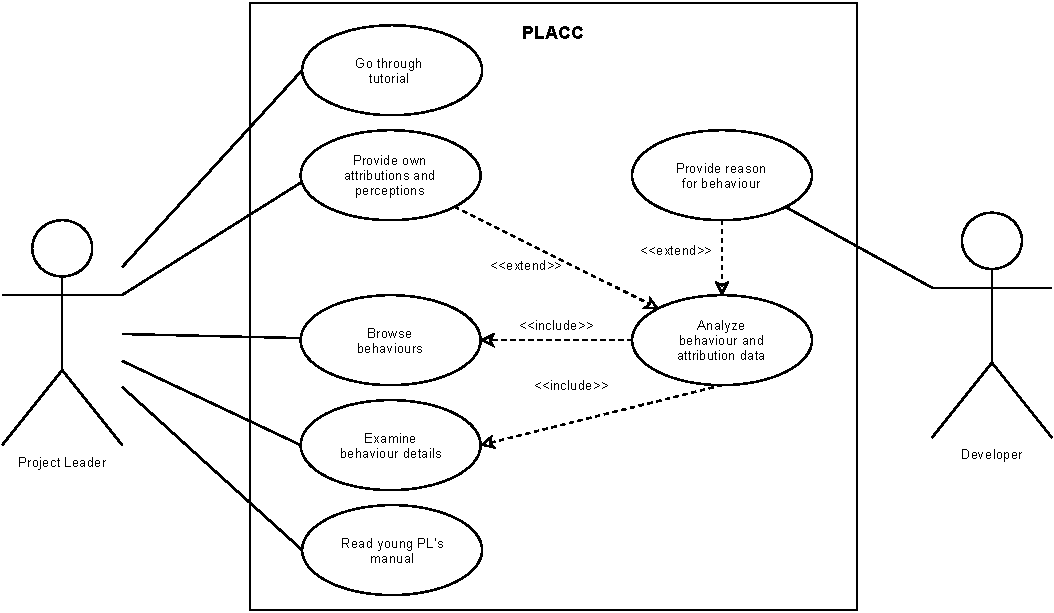
\includegraphics[width= \textwidth]{figures/UseCaseModel.pdf}
	\caption{Use Case Model}
	\label{fig:UseCaseModel}
\end{figure}

\subsection{Analysis Object Model}

%\textit{Note: This subsection should contain a UML Class Diagram showing the most important objects, attributes, methods and relations of your application domain including taxonomies using specification inheritance (see \cite{bruegge2004object}). Do not insert objects, attributes or methods of the solution domain.
%\textbf{Important:} Make sure to describe the analysis object model thoroughly in the text so that readers are able to understand the diagram. Also write about the rationale how and why you modeled the concepts like this.}

\begin{figure}
	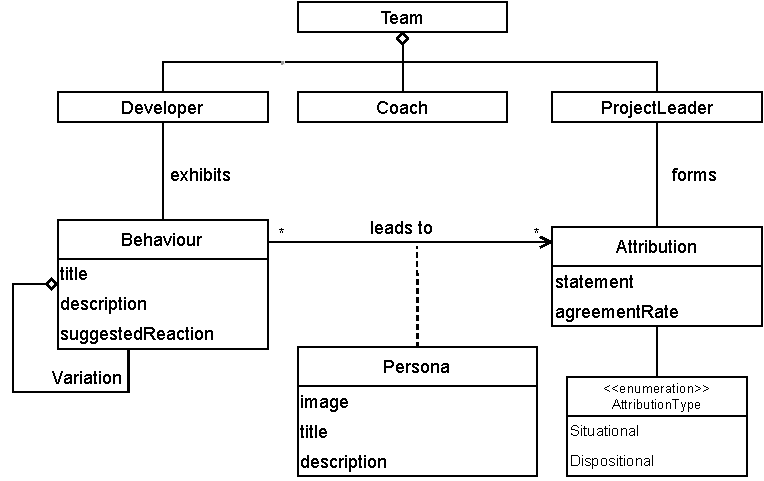
\includegraphics[]{figures/AOM2.pdf}
	\caption{Analysis Object Model}
	\label{fig:AOM}
\end{figure}

~\autoref{fig:AOM} depicts the \textit{Analysis Object Model (AOM)} of the system under development. The AOM represents the main objects and the relationships that exist among them from the user's point of view. As specified in \cite{bruegge2004object}, the AOM serves as a visual dictionary of the concepts participating in the system.

Not only the AOM but also the ideation of this thesis started from observing agile software development \textbf{teams} and the dynamics that emerge between its participants. The team we observe are distributed and operate using means of remote communication and collaboration. Meetings are held on Zoom, communication takes place in platforms such as RocketChat or Discord and screensharing and remote control facilitate group collaboration especially in development tasks. The team follows the structure, guidelines and processes of Scrum \footnote{https://www.scrum.org/resources/what-is-scrum}.

The iPraktikum teams consist of the \textbf{project leader}, \textbf{coach} and \textbf{the developers}. The project leader serves as the product owner and is responsible for communicating and reinforcing the product goals into the team. The coach represents the scrum master, and makes sure that the scrum principles are maintained. The scrum developers are responsible for providing increments until eventually building the product. In the semester in which this case study took place, there were 1-2 project leaders and coaches per team. 

Although every human being acts and expresses oneself via \textbf{behaviours}, we are specifically interested in the ones exhibited by the developers of the team. We consider the relation between the developers and the project leaders the more interesting to observe, as their competences are distinct and as the project leader has a more distant relationship to the team. This is contrasting to the position of the coach, who needs to stay closer to team.

After the interviews with the project leaders and the process of building a taxonomy of behaviours, it was identified that, although some behaviours were similar in their core, they could also vary depending on the context or circumstances. This taxonomy was constructed as an attempt to understand the domain, and we concluded that broader behaviours consist of more specific \textbf{variations}.

We judged that a behaviour consists of a title, a description and a suggested reaction towards this behaviour. Normally a behaviour is characterized by numerous other properties, but these three are the ones we consider.

Other important properties such as motivation or reason of a behaviour are not studied directly, but rather indirectly as part of the \textbf{attributions} project leaders form. Similarly to behaviours, everyone is capable of forming attributions, but the project leaders are taken into consideration as the subjects of the study. Attributions are formed as a developer exhibits a behaviour, usually new or different from what the perceiver (in our case the PL) is used to see. 

An attribution is expressed by a statement, and embodies the reasoning behind the causes of a behaviour. Considering that the survey described in \autoref{chap:Survey} also served the validation and quantification of attributions, we were able to retrieve the frequency of the agreeing responses to each attribution. Although we have retrieved other metrics in regards to an attribution, the agreement rate is the one we deemed as interesting for the users of PLACC. The agreement rate makes it possible to identify \textbf{personas} too.

An attribution can be situational or dispositional. If the \textbf{attribution type }is situational, it means that the project leaders take in consideration the situation and circumstances of the developer when forming an attribution. Dispositional attribution happens, when the disposition of the developer is considered as the cause of a behaviour. The disposition included character, personality and demeanour.

A behaviour can lead to multiple attributions, and a attribution (e.g. bad internet connection) can be used as an excuse to many behaviours. In this system we focus rather on the first association between the two objects, hence, the unidirectional arrow in the model. 

In the intersection of behaviours and attributions is where \textbf{personas} will be found. A persona is a personification of an individual which exhibits a certain set of behaviours, and is perceived a specific way by the project leaders. A persona has a title, usually a short and striking one, and a description that gives more details. An image is also associated with a persona, is order to add a visual element as well.   

\subsection{UI Mockups}

\begin{longtable}[ht]{ p{0.45\textwidth}  p{0.45\textwidth} }
\caption{UI Mockups}
\label{tab:mockups}\\
\hline
\textbf{Browse behaviours} & \textbf{Explore behaviour details} \\
    \hline
   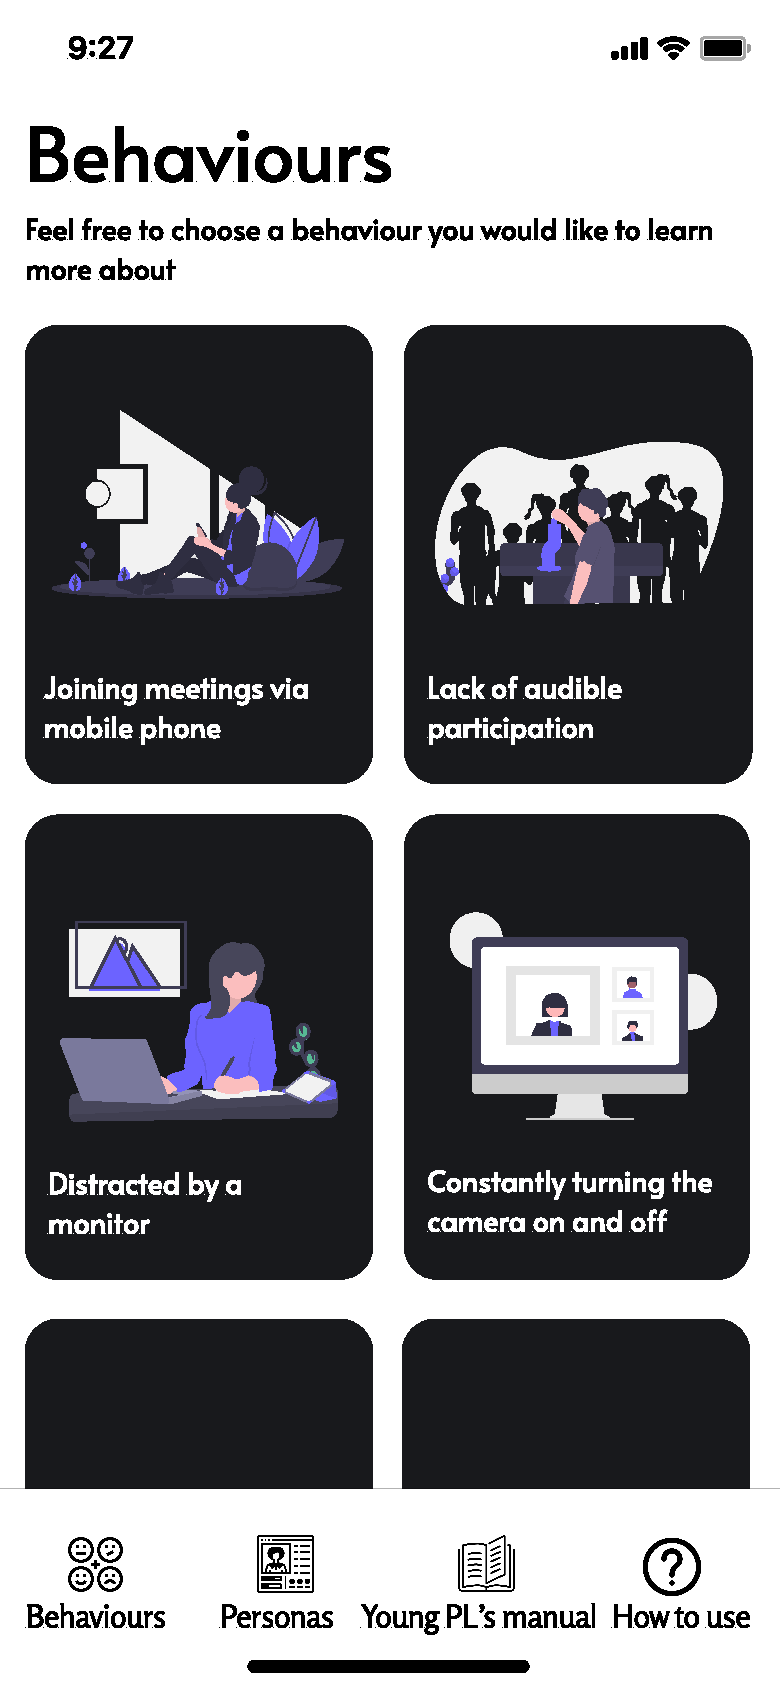
\includegraphics[valign=t, width=2in]{figures/Behaviours.pdf} &   		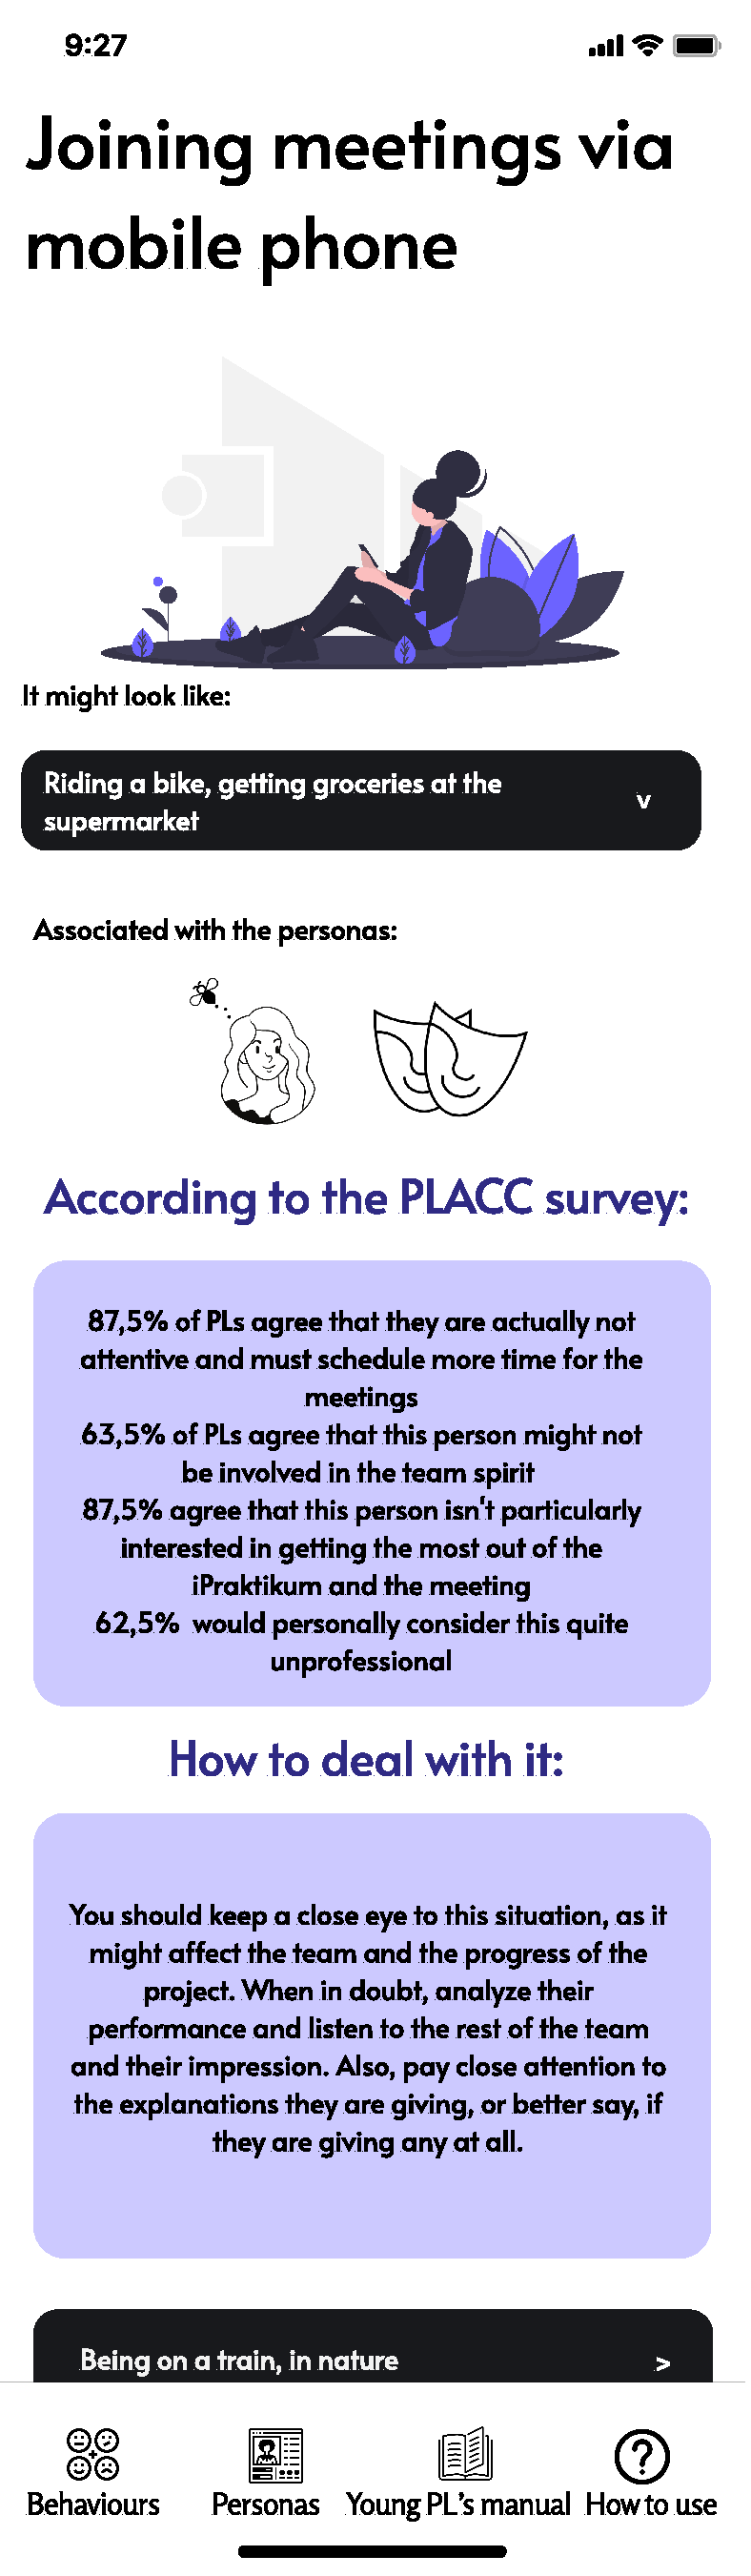
\includegraphics[valign=t, width=2in]{figures/ASpecificBehaviour.pdf} \\
   \hline
   Description1  &  Description2  \\
   \hline
   \textbf{Personas} & \textbf{Young PL Manual}\\
    \hline
   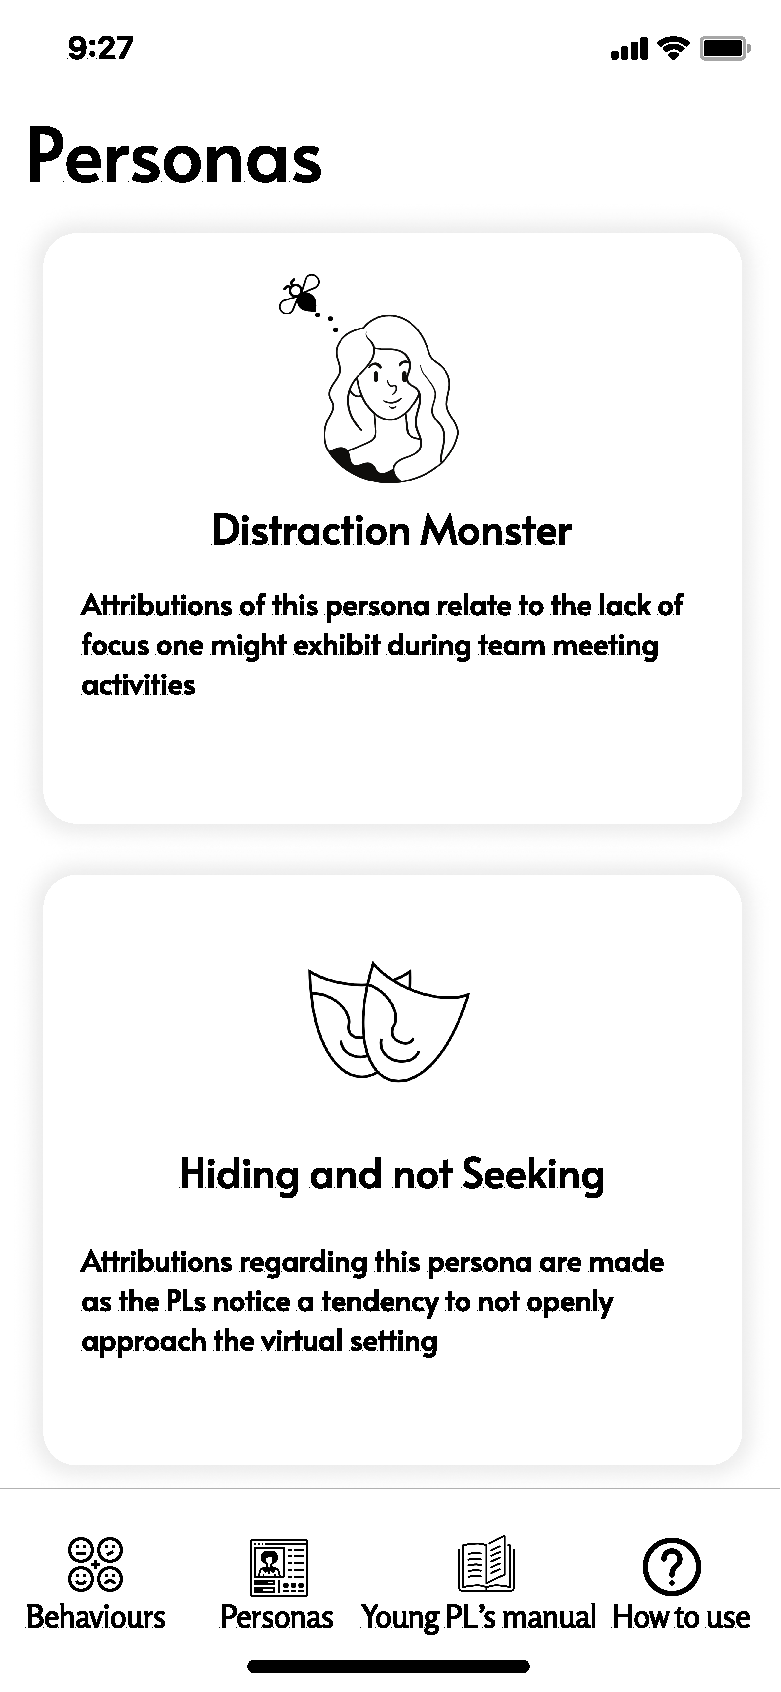
\includegraphics[valign=t, width=2in]{figures/Personas.pdf} &   		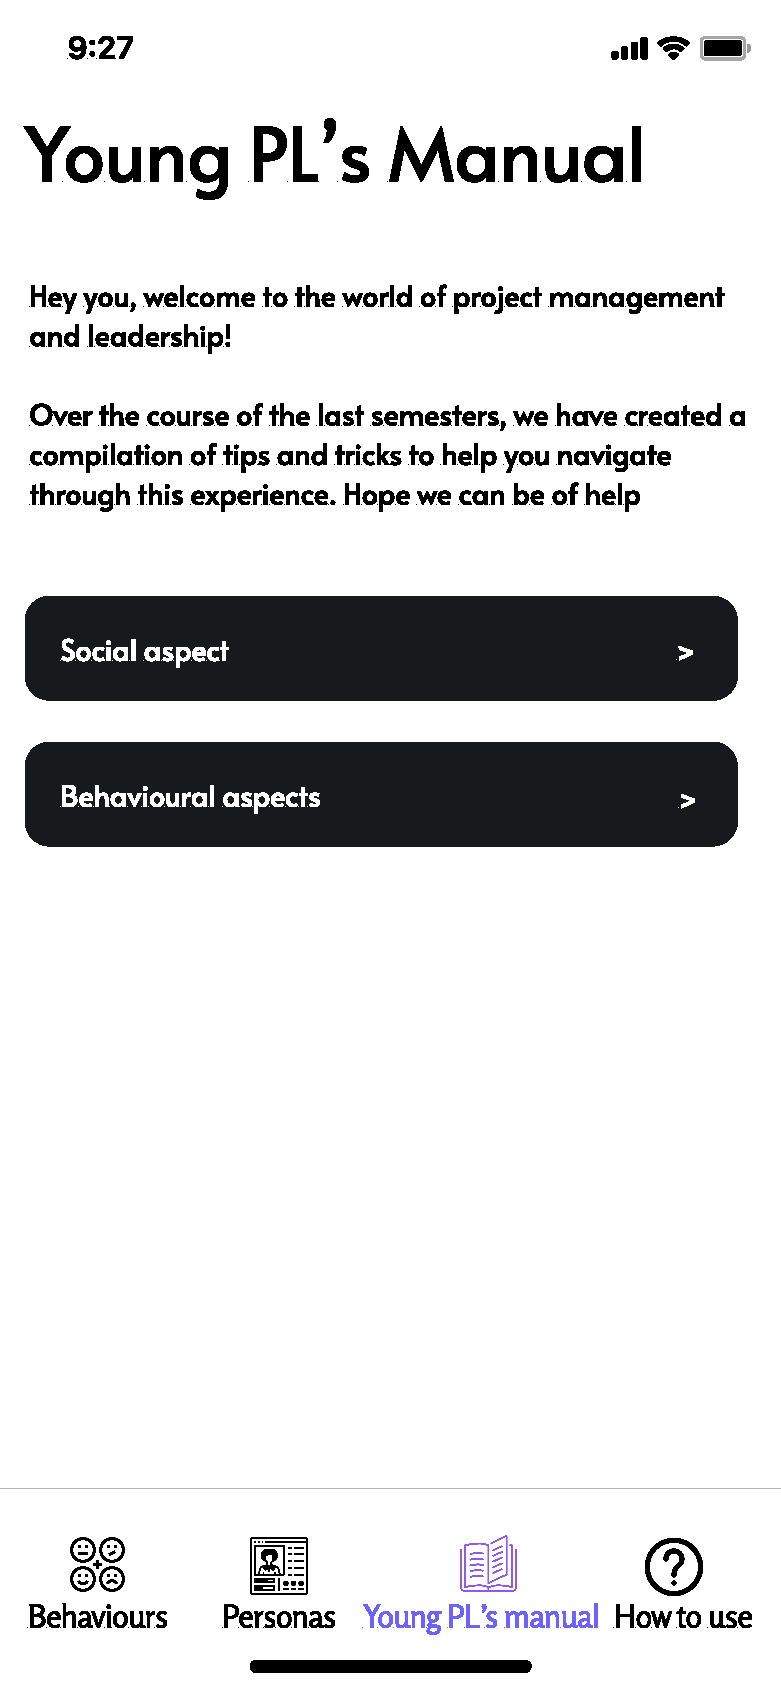
\includegraphics[valign=t, width=2in]{figures/HowTo.pdf} \\
   \hline
   Description3  &  Description4  \\
   \hline
\label{tab:multicol}
\end{longtable}


